\documentclass{whutmod}
\usepackage{metalogo}
\usepackage{float}
\usepackage{subfigure} 
\usepackage{url}
\usepackage{booktabs}
\bibliographystyle{unsrt}
\team{23}
\membera{刘子川}
\joba{编程}
\memberb{程宇}
\jobb{建模}
\memberc{陈荣兴}
\jobc{建模}
\hypersetup{
	colorlinks=true,
	linkcolor=black
}

\title{基于因子分析与灰色关联分析对武汉市人才吸引力的量化评价}
\tihao{4} 

\begin{document}

	%\maketitle
	
	\begin{abstract}

城市的发展对人才的吸引力两者之间是相互联系与制约的,因此需要政府决策与措施影响,使城市增强对人才的吸引力。本文结合武汉的发展特点,利用\textbf{爬取}后的数据较全面的选择合适的指标进,通过\textbf{因子分析}的方法为武汉市不同年份人才吸引力打分;再对人才进行产业类别分类,通过\textbf{灰色关联分析}筛选出合适的因子后再横向比较各城市综合得分,并结合当地人才政策评价对人才吸引力的水平提出合理化建议。
~\\%~\\为换行

针对问题一,通过\textbf{因子分析模型}分析武汉2013—2017年相关数据,对武汉各年的人才吸引力进行\textbf{量化打分}。本组首先根据题目要求和以往人才吸引要素研究,确立要素框架并\textbf{爬取}合适的人才吸引力因素。在标准化数据通过\textbf{KMO检验}后,利用SPSS对各个因素进行\textbf{主成分分析}以确定公因子数目,求解旋转后因子荷载矩阵并对公因子命名,计算武汉各年人才吸引力综合得分。综合得分结果为\textbf{-77.99、-30.08、-11.90、42.35、77.63}。综合得分表明武汉2013—2017人才吸引力逐年上升,且2015—2016年上升幅度最大,与城市实际发展情况相符合。
~\\

针对问题二,本文在问题一模型的基础上进行改进,将人才分为第一、第二和第三产业人才并用\textbf{灰色关联分析}筛选出每类人才相应的人才吸引力因素。然后将筛选后的数据用SPSS进行\textbf{因子分析}得到成都、天津、西安、南京和武汉2013—2017年的三类人才吸引力因子分析模型,并计算每个城市各年针对三类人才的人才吸引力\textbf{综合得分}。横向比较各个城市的综合得分,相较与其他城市,武汉市近几年对第二、三产业人才的吸引力有较高水平,相对于西安和成都,武汉市具有较强的人才吸引力,符合地区的经济发展特点。
~\\

针对问题三,基于问题一中的武汉市人才吸引力评价模型以及人才政策对人才吸引力的量化评价,并结合问题二中武汉相较于其他四个同类城市在人才吸引力上的优势与不足,给武汉市人力资源管理部门的领导写一篇建议报告。
~\\

本文中所提到的模型优点主要有两点:一、选取的指标从多维度、全方面考虑,收集的数据真实可靠;二、利用灰色关联度筛选出三类人才的人才吸引力要素,相较于人工选取指标具有客观性、严谨性。
  
\keywords{因子分析模型\quad  主成分分析\quad  灰色关联分析\quad 数据库爬虫\quad }
		
	\end{abstract}
	
	%目录
	\tableofcontents
	\newpage	%换页符
	
	\section{问题重述}	
	\subsection{问题背景}
    植物的种类繁多,要了解和掌握如此多的植物,必须进行一个科学的分类。人们常常根据植物的用途,或根据植物的一个或几个明显的形态进行分类,植物的识别与分类对于区分植物种类,探索植物间的亲缘关系,阐明植物系统的进化规律具有重要的意义。因此植物分类学是植物科学甚至整个生命科学的基础学科。目前对于树叶识别与分类主要由人完成,但是树叶种类庞大,依赖人工地进行树叶识别与分类是不现实的。所以树叶的研究对于植物总体的研究能提供很大的帮助。
    
    从树叶的各个方面,纹理,硬度,离心率等方面都可作为主要方向研究,现对树叶的研究主要通过采集树叶图形,利用数字图像处理来对树叶进行分类识别,这种方法只停留在处理形态特征,有很大的局限性,忽略了树叶的生理特征和其他特征,所以研究方法来综合处理树叶平面图像特征,形态特征和生理特征很有必要性。
    
    

	\subsection{问题提出}
    围绕植物分类进行树叶识别与分类,以树叶二值化图片为依据,依次提出以下问题:
		 
	\begin{itemize}
	\item [(1)] 结合附件中的二值化的图片数据,建立合适的图片数据提取方案, 量化处理图片数据,并具体分析说明所提取数据信息的量化指标体系。
	\item [(2)] 基于问题一中提取的数据信息,建立合适的数学模型由数据出发判断叶子的种类,研究判别分类的核心指标,并估计出模型的性能以及核心指标对模型判别性能的影响。
	\item [(3)] 基于二值化图片数据,结合附件中叶子纹理的数据信息,对原有模型进行改进,并对新旧模型进行比较分析。
	\end{itemize}
	
	\section{模型假设}
	\begin{itemize}
		\item [(1)] 假设相同的行业在不同的城市里吸引力影响因素相同,每个行业在不同城市里的发展模式近似相同。
		\item [(2)] 人才会考虑未来一段时间内自身对于发展前景、收入、环境的需求的变化。
		\item [(3)] 政策对人才吸引力的影响转换成三个影响因素——地方财政支出与收入和固定资产投资总额。
		\item [(4)] 人才的迁移是在追求效用最大化,人才的行为仅受到城市因子的影响,忽略人的非理性行为。
	\end{itemize}
	
	
	\section{符号说明}
%	每行都有线的表
%	\begin{center}
%		\begin{tabular}{cc}
%			\hline
%			\makebox[0.3\textwidth][c]{符号}	&  \makebox[0.4\textwidth][c]{意义} \\ \hline
%			$C_{0}$	    &  污染源初始浓度 \\ \hline
%			$C(x,t)$	    &  污染浓度随时空变化 \\ \hline
%			$u_{x}$	    &  江河平均纵向流速 \\ \hline
%			$E_{x}$  &  铊在江河纵向弥散系数\\ \hline
%		$p$   &  面污染物纵向距离\\ \hline
%			$K_{c}$	    & 污染物降解系数  \\ \hline
%		    $a$	& 污染超标系数 \\ \hline
%		     $x$	& 距污染源的一维距离 \\ \hline
%		      $t$	& 距污染发生后的时间 \\ \hline
%		       $V_{A}$	& 溶液摩尔体积 \\ \hline
%		      $M_{B}$	& 江水的摩尔质量 \\ \hline
%		     $\mu_{B}$	& 溶剂的粘度 \\ \hline		      
%		\end{tabular}
%	\end{center}

%三线表
	\begin{table}[H]
	\label{biao} \centering
		\begin{tabular}{cc}
			\toprule[1.5pt]
			\multicolumn{1}{m{5cm}}{\centering 符号} & \multicolumn{1}{m{5cm}}{\centering 说明} \\
			\midrule[1pt]
			$F$	 &  城市各年人才吸引力综合得分  \\ 
			$F_{1}$ &  工业发展与薪酬因子 \\ 
			$F_{2}$	 &  医疗卫生环境因子 \\ 
			$F_{3}$  &  经济贸易因子 \\ 
			$F_{4}$  &  拥挤程度因子 \\ 
			$X$  &  原始指标 \\ 
			$\overline{X}$  &  指标平均值 \\ 
			$\widetilde{X}$  &  同向化指标 \\ 
	     	$\delta_{X}$  &  指标标准差 \\ 
	     	$Z$  & 标准化指标 \\ 
	     	$R$  & 相关系数矩阵 \\ 
	     	$\lambda_{p}$  & 相关系数矩阵特征值 \\ 
	     	$\eta _ {p}$  & 标准正交化特征向量 \\ 
	     	$\Lambda$ & 因子载荷矩阵 \\ 
	     	$\sigma_{i}$ & 方差 \\
	     	$\alpha_{i j}$ & 载荷因子 \\
	     	$k$ & 两极最小差 \\
	     	$K$ & 两极最大差 \\
	     	$\Delta _{i}(t)$ & 特征序列与因素序列的序列差 \\
			\bottomrule[1.5pt]
		\end{tabular}
	\end{table}

	\section{问题一模型的建立与求解}
	\subsection{问题的描述与分析}

	针对问题一,本题要求建立合适方案提取二值化图片中的数据,并对所提取数据的量化指标进行分析说明。本组通过解析几何计算和时间序列展开,将目标图像转化成两个特征向量。本组根据题目要求和近年的图像识别研究,确定了针对二值化图像的两个重点识别因素——轮廓特征因素和边缘特征因素。针对轮廓特征因素,首先利用matlab做解析几何运算,计算与图像轮廓有关的特征量,并将计算结果作为元素,组成轮廓特征向量。针对边缘特征因素,首先将图像边缘通过极化投影展开为时间序列,计算每支时间序列的特征量,并将计算结果作为元素,组成边缘特征向量。最后合并两个向量得到总体特征向量。
	    \subsection{模型的建立}
	    \subsubsection{图像基本参数定义}
		定义$I$表示目标树叶所对应的图像,$\partial I$表示图像边界,$D(I)$表示图像最小外接圆直径,$d(I)$表示图像最大内切圆半径,$A(I)$表示研究对象面积,$L(\partial I)$表示研究对象的轮廓线长度,$H(I)$表示研究对象的凸包域,$C(I)$为图像几何中心坐标,运算符$d(.)$代表欧式距离。
	    \subsubsection{轮廓特征因素}
		定义轮廓特征向量为$ID1_{1}=[id_{1},id_{2},\cdots,id_{n}](n=6)$其中$id_{k}(k=1,2,\cdots,6)$为二值化矩阵的轮廓特征,其具体计算公式如下:
		\begin{itemize}	
		\item [$id_{1}$]长宽比(Aspect Ratio):
		定义$X_{I}$为图像最上方非零行与最下方非零行的行数差(长),$Y_{I}$为图像最左方非零列与最右方非零列的列数差(宽),长宽比$id_{1}=X_{I}/Y_{I}$。
		
		\item [$id_{2}$]离心率(Eccentricity): 
		定义$E(I)$是与研究图像具有相同的二阶矩的椭圆,$a$和$b$分别为$E(I)$对应的长轴与短轴,离心率$id_{2}=\sqrt{1-(\frac{b}{a})^{2}}$,变化范围为(0,1)。
		
		\item[$id_{3}$]密实度(Solidity):
		实密度$id_{3}=\frac{ A }{A(H(I))}$。其反映研究对象的仿射特征,即研究对象区域的固靠性程度。
		
		\item [$id_{4}$]等周因子(Isoperimetric Factor):
		等周因子$id_{4}=\frac{4\pi \cdot  A}{L(\partial I)^{2}}$ ,其变化范围为(0,1),描述目标树叶轮廓规整度,叶子边缘越规则,其值越接近于最大值1。
		
		\item [$id_{5}$]伸长率(Elongation): 
		伸长率$id_{5}=1-\frac{2d_{I}}{D(I)}$,变化范围为(0,1),树叶越趋于圆形,相应的伸长率越小,比率$\frac{2d_{max}}{D(I)}$ 其描述目标树叶轮廓向外伸展的趋势。
		
		\item[$id_{6}$]最大压痕深度(MaximalIndentationDepth):
		定义$C_{H(I)}$为研究对象凸型区域的几何中心,$L(\partial I)$表示为$H(I)$的轮廓线长度,$\forall X\in H(I)$和$\forall Y\in \partial I$,计算距离$d(X,C_{H(I)})$和$d(Y,C_{H(I)})$。定义函数$\frac{ d(X,C_{H(I)})- d(Y,C_{H(I)})}{L(H(I))}$,该函数的最大值即最大压痕深度$id_{6}$。
		
		
		\subsubsection{边缘特征因素}
		为得到研究对象的边缘特征,首先以$C(I)$为坐标原点建立笛卡尔坐标系,对于曲线$\partial I$上任意一点$P$可以在该坐标系下表示为$P(x_{p},y_{p})$,将其投影至以$C(I)$为极点的极坐标系得${P}'(r_{p},\theta _{p})$,其中:
		\begin{gather}
		r_{p}=d(P(x_{p},y_{p}).C(I))
		\end{gather}
		\begin{gather}
		\theta _{p}=y_{p}/x_{p},
		\end{gather}
		(图1)
		通过将点集${{P}'(r_{p},\theta _{p})}$降维可得到时间序列$arrays({P}')$。将arrays滤波处理后,计算每支时间序列上的极大值点数$id_{7}$,极小值点数$id_{8}$。得到边缘特征向量$ID2=[id_{7},id_{8}]$,合并轮廓特征向量与边缘特征向量得:
		\begin{gather}
		ID=[ID1,ID2]
		\end{gather}
	     其中ID为总体特征向量。
	      \subsection{模型的求解}
	      首先使用matlab围绕regionprops函数对研究对象进行解析几何计算,用遍历式算法逐一算出研究对象长宽比、离心率、实密度、等周因子、伸长率和最大压痕深度,得到轮廓特征向量(见代码?)。再将图片通过numpy工具箱标准正立化,以其几何中心为极点将其边缘坐标转换为极坐标,然后使用ndarrays函数将所得极坐标降维展开成时间序列,搜寻滤波后时间序列的极点数得到边缘特征向量。
	     
		\subsubsection{}
		根据标准化处理后的指标数据,利用$SPSS23.0$统计软件进行$KMO$和巴特利特检验,以确认所选变量是否适合做因子分析,结果如表\label{tab1}所示:
		% Table generated by Excel2LaTeX from sheet 'Sheet1'
		\begin{table}[H]
			\centering
			\caption{KMO和Bartlett的检验}\label{tab1}
			\begin{tabular}{cc|cc|cc}
				\toprule[1.5pt]
				\multicolumn{4}{c|}{取样足够度的Kaiser-Meyer-Olkin度量} & \multicolumn{2}{c}{0.859} \\
				\midrule
				\multicolumn{2}{c|}{\multirow{3}[2]{*}{Bartlett的球形度检验}} & \multicolumn{2}{c|}{近似卡方} & \multicolumn{2}{c}{1183.981} \\
				\multicolumn{2}{c|}{} & \multicolumn{2}{c|}{df} & \multicolumn{2}{c}{78} \\
				\multicolumn{2}{c|}{} & \multicolumn{2}{c|}{Sig.} & \multicolumn{2}{c}{.000} \\
				\bottomrule[2pt]
			\end{tabular}%
			\label{tab:addlabel}%
		\end{table}%
		
		由上表可知,巴特利特球度检验统计量的观测值为$1183.981$,相应的概率$P$值接近$0$。若显著性水平$α$为$0.5$,概率$P$小于显著性水平$α$,应拒绝零假设,认为相关系数矩阵与单位阵有显著差异,即因子协方差矩阵不是单位阵。同时,$KMO$值为$0.859$,$KMO>0.8$,根据$KMO$ 度量标准可知原有变量适合进行因子分析。
		
		
		

	\subsection{模型的建立与求解}
	\subsubsection{公因子的确定}
	根据上述指标标准化后,其对应相关系数矩阵部分数据见表~\ref{shuju2}~所示(详见附录):
	%三线表
	\begin{table}[H]
		 \centering
		\caption{相关系数矩阵部分数据}\label{shuju2}
		\begin{tabular}{ccccccc}
			\toprule[2pt]
			\multicolumn{1}{m{1cm}}{\centering } &
			\multicolumn{1}{m{2cm}}{\centering $X_{1}$} & \multicolumn{1}{m{2cm}}{\centering $X_{2}$} & \multicolumn{1}{m{2cm}}{\centering $X_{3}$}&
			\multicolumn{1}{m{2cm}}{\centering $X_{4}$}&
			\multicolumn{1}{m{1cm}}{\centering ........} &
			\multicolumn{1}{m{2cm}}{\centering $X_{33}$}
			\\
				\midrule[1pt]
			$X_{1}$&1.000	 &  0.727 & -0.423&0.967&........& -0.928\\ 
			$X_{2}$& &  1.000 & -0.796&0.822&........&-0.814\\ 
			$X_{3}$& &   & 1.000&-0.620&........&0.682\\ 
			$X_{4}$& &   & &1.000&........&-0.955\\ 
			........& &   & & &........&........\\ 
			$X_{33}$& &   & & &........&1.000\\
			\bottomrule[2pt]
		\end{tabular}
	\end{table}
	
	设$\lambda_{1} \geqslant \lambda_{2} \geqslant \cdots \geqslant \lambda_{p}$为样本相关系数矩阵$R$的特征值,$\eta _ { 1 } , \eta _ { 2 } , \cdots , n _ { p }$为相应的标准正交化特征向量。设$m<p$,则因子载荷矩阵$\Lambda$为:
	\begin{gather}
	\Lambda=\left[\sqrt{\lambda_{1}} \eta_{1}, \sqrt{\lambda_{2}} \eta_{2}, \cdots, \sqrt{\lambda_{m}} \eta_{m}\right]
	\end{gather}
    用$\boldsymbol{R}-\boldsymbol{\Lambda} \boldsymbol{\Lambda}^{\mathrm{T}}$对角元来估计特殊因子的的方差:
	\begin{gather}
	\sigma_{i}^{2}=1-\sum_{j=1}^{m} \alpha_{i j}^{2}
	\end{gather}
	式中:$\sigma_{i}$为方差,$\alpha_{ij}$表示载荷因子。由上述分析,得总方差解释部分数据如表~\ref{biaosan}~所示:	
		\begin{table}[H]
		\centering
		\caption{总方差解释}\label{biaosan}
		\begin{tabular}{ccccccc}
			\toprule[1.5pt]
		\multicolumn{1}{m{1cm}}{\centering } &
				\multicolumn{1}{m{1.5cm}}{\centering  } &
		 \multicolumn{1}{m{3cm}}{\centering 初始特征值} &
		 		\multicolumn{1}{m{1cm}|}{\centering  } &
		\multicolumn{1}{m{1cm}}{\centering  } &
		 \multicolumn{1}{m{3cm}}{\centering 提取载荷平方和}&
		 		\multicolumn{1}{m{1.5cm}}{\centering  } \\\hline
		\multicolumn{1}{m{1cm}|}{\centering  成分} &
		\multicolumn{1}{m{1.5cm}}{\centering  总计} &
		\multicolumn{1}{m{3cm}}{\centering  方差百分比} &
		\multicolumn{1}{m{1cm}|}{\centering  累积} &
		\multicolumn{1}{m{1cm}}{\centering  总计} &
		\multicolumn{1}{m{3cm}}{\centering  方差百分比} &				\multicolumn{1}{m{1.5cm}}{\centering  累积} \\

			\midrule[1pt]
			1&25.330&76.758&76.758&25.330&76.758&76.758 \\
			2&4.025&12.197&88.956&4.025&12.197&88.956 \\
			3&2.373&7.191&96.147&2.373&7.191&96.147 \\
			4&1.271&3.852&99.920&1.271&3.852&99.920 \\
			5&5.129e-15&1.554e-14&100.0&&& \\
			6&1.330e-15&4.031e-15&100.0&&& \\
			7&6.062e-16&1.837e-15&100.0&&& \\
			8&5.067e-16&1.535e-15&100.0&&& \\
			9&4.532e-16&1.373e-15&100.0&&& \\
			10&3.335e-16&1.011e-15&100.0&&& \\
			11&3.137e-16&9.506e-16&100.0&&& \\
			12&2.585e-16&7.834e-16&100.0&&& \\
			13&1.990e-16&6.031e-16&100.0&&& \\
			......&......&.......&100.0&&& \\
			......&......&.......&100.0&&& \\
			33&-2.279e-15&-6.908e-15&100.0&&& \\
			\bottomrule[1.5pt]
		\end{tabular}
	\end{table}
	
	
	由表~\ref{biaosan}~特征根知,因子$F_{1}$的特征值$\lambda_{1}=25.330$,占方差的 $76.75\%$。由碎石图~\ref{123}~可知,当提取$1,2$个公因子时,特征值变化非常明显,当提取第$5$个以后的公因子时,特征值变化比较小,基本趋于平缓。由此说明,提取$4$个公因子对原变量信息的刻画有显著作用。因此,在这里我们提取$4$个公共因子,这$4$个公因子的累计方差达到$99.92\%$,即这$4$个公因子可以反映原来$33$个指标的$99.92\%$的信息量,可见采用前\textbf{4个公因子}对武汉2013—2017年人才吸引力进行评价是比较合适的。
	
	\begin{figure}[H]
		\centering
		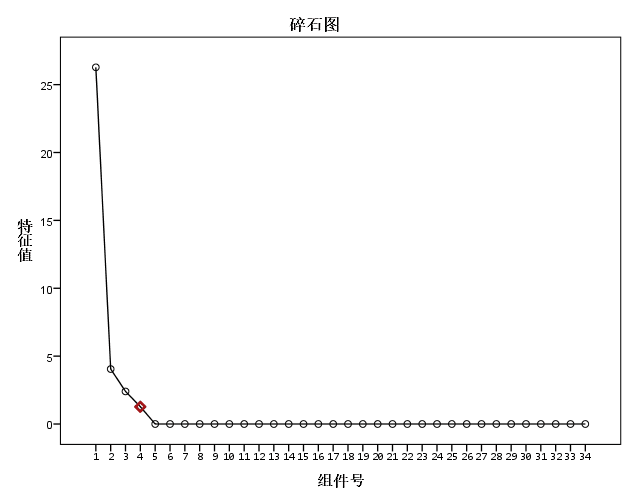
\includegraphics[width=\textwidth]{figures/123.png}
		\caption{碎石图}\label{123}
	\end{figure} 
	
	\subsubsection{因子命名与载荷矩阵计算}

	表~\ref{cehngfenjuzheng}~是初始因子载荷矩阵(详见附录),由此可写出因子分析模型的如下:
	\begin{gather}
	\begin{array} { l } { \mathrm { X } _ { 1 } = 0.989 \mathrm { F } _ { 1 } + 0.123 \mathrm { F } _ { 2 } - 0.074 \mathrm { F } _ { 3 } - 0.031 \mathrm { F } _ { 4 } } \\ { \mathrm { X } _ { 2 } = 0.795 \mathrm { F } _ { 1 } - 0.556 \mathrm { F } _ { 2 } - 0.193 \mathrm { F } _ { 3 } - 0.151 \mathrm { F } _ { 4 } } \\ { \ldots \ldots } \\ { \mathrm { X } _ { 33 } = - 0.958 \mathrm { F } _ { 1 } + 0.176 \mathrm { F } _ { 2 } - 0.060 \mathrm { F } _ { 3 } + 0.220 \mathrm { F } _ { 4 } } \end{array}
	\end{gather}
			\begin{table}[H]
	\centering
	\caption{初始因子载荷矩阵}\label{cehngfenjuzheng}
	\begin{tabular}{ccccc}
		\toprule[2pt]
		\multicolumn{1}{m{2cm}}{\centering 指标} &
		\multicolumn{1}{m{1cm}}{\centering $F_{1}$} & \multicolumn{1}{m{1cm}}{\centering $F_{2}$} & \multicolumn{1}{m{1cm}}{\centering $F_{3}$}&
		\multicolumn{1}{m{1cm}}{\centering $F_{4}$}\\
		\midrule[1pt]
		地方财政预算支出&0.989	 & 0.123 & -0.074&-0.031\\ 
		固定资产总额&0.795 &-0.556 &-0.193&0.151\\ 
		年末邮政局数&-0.548 &0.768  &-0.333&0.008\\ 
		执业医师人数&0.994 &-0.027 &-0.245 &0.002\\ 
		........& ........&  ........ &........ &........ \\ 
		年末固定电话数&-0.958 &-0.176   &-0.060 &0.220 \\
		\bottomrule[2pt]
	\end{tabular}
\end{table}
		表~\ref{cehngfenjuzheng}~中的每个数据表示了相应因子变量对相应原变量的相对重要程度。由于得到的公共因子与各指标的载荷分布归类比较困难,需要对因子载荷矩阵进行正交旋转,这里运用方差最大正交旋转法\cite{宋鸿2010城市人才吸引力的影响因素及提升对策},得到旋转后的因子载荷矩阵表~\ref{xuanzhuanhuo}~所示(详见附录):
			\begin{table}[H]
			\centering
			\caption{旋转后的因子载荷矩阵}\label{xuanzhuanhuo}
			\begin{tabular}{ccccc}
				\toprule[2pt]
				\multicolumn{1}{m{2cm}}{\centering 指标} &
				\multicolumn{1}{m{1cm}}{\centering $F_{1}$} & \multicolumn{1}{m{1cm}}{\centering $F_{2}$} & \multicolumn{1}{m{1cm}}{\centering $F_{3}$}&
				\multicolumn{1}{m{1cm}}{\centering $F_{4}$}\\
				\midrule[1pt]
				地方财政预算支出&0.870	 & 0.356 & 0.076&0.331\\ 
				固定资产总额&0.469 & 0.311 &0.678&0.473\\ 
				年末邮政局数&-0.291 & -0.390  &-0.867&0.105\\ 
				执业医师人数&0.787 &0.496   &0.259 &0.259\\ 
				........& ........&  ........ &........ &........ \\ 
				年末固定电话数&-0.872 &-0.277   &-0.384 &-0.124 \\
				\bottomrule[2pt]
			\end{tabular}
		\end{table}
	
	根据表~\ref{xuanzhuanhuo}~发现,旋转在\textbf{9次迭代}后已收敛。旋转后的因子系数已经明显向两极分化,有了更鲜明的实际意义。因子载荷的绝对值越大,则表明该因子与变量的重叠性越高,在解释因子的时候就越重要。

		第一因子$F_{1}$主要包含地区生产总值、第一第二产业生产总值、在岗职工平均工资和人均GDP等,这些指标包含了地区工业发展水平以及人均薪酬水平故将其命名为\textbf{工业发展与薪酬因子}。第二因子$F_{2}$主要包含持证医师人数,医院卫生院个数以及一年内空气质量达到及好于二级的天数等,这些指标包含了地区医疗卫生水平和居民生活环境,故将其命名为\textbf{医疗卫生环境因子}。第三因子$F_{3}$主要包含固定资产投资总额与货物进出口总额,该指标反映了城市贸易与经济发展水平,故将其命名为\textbf{经济贸易因子}。第四因子$F_{4}$包含年末总人口与旅游生产总值,反映了城市人口与拥挤程度故将其命名人口与\textbf{拥挤程度因子}。

	\subsubsection{求得因子得分和综合绩效得分}
	采用回归法估计因子得分系数,并输出因子得分系数矩阵,其结果见表~\ref{defenyinzi}~所示(详见附录):
				\begin{table}[H]
		\centering
		\caption{成分得分系数矩阵}\label{defenyinzi}
		\begin{tabular}{ccccc}
			\toprule[2pt]
			\multicolumn{1}{m{2cm}}{\centering 指标} &
			\multicolumn{1}{m{1cm}}{\centering $F_{1}$} & \multicolumn{1}{m{1cm}}{\centering $F_{2}$} & \multicolumn{1}{m{1cm}}{\centering $F_{3}$}&
			\multicolumn{1}{m{1cm}}{\centering $F_{4}$}\\
			\midrule[1pt]
			地方财政预算支出&0.052 & -0.017 & -0.021&0.024\\ 
			固定资产总额&-0.063 & 0.045 &0.127&0.137\\ 
			年末邮政局数&0.022 &-0.079  &-0.195&0.109\\ 
			执业医师人数&0.007 &0.064 &0.021 &0.009\\ 
			........& ........&  ........ &........ &........ \\ 
			年末固定电话数&-0.109 &0.093 &-0.068 &0.094 \\
			\bottomrule[2pt]
		\end{tabular}
	\end{table}
	则根据表~\ref{defenyinzi}~可以计算出四个主因子得分,表达式分别为:
	\begin{gather}
	\begin{matrix}
	F_{1}=0.052x_{1}-0.063x_{2}+0.022x_{3}+0.007x_{4}+\cdots-0.109x_{33}\hfill\\ 
	F_{2}=-0.017x_{1}+0.045x_{2}-0.079x_{3}+0.064x_{4}+\cdots+0.093x_{33}\hfill\\ 
	F_{3}=-0.021x_{1}+0.127x_{2}-0.195x_{3}+0.021x_{4}+\cdots-0.068x_{33}\hfill\\ 
	F_{4}=0.024x_{1}+0.137x_{2}+0.109x_{3}+0.009x_{4}+\cdots+0.094x_{33}\hfill
	\end{matrix}
	\end{gather}
	
	利用SPSS软件计算得到旋转后的因子贡献及贡献率如表~\ref{fff}~所示:
			\begin{table}[H]
	\centering
	\caption{旋转后因子贡献及贡献率}\label{fff}
	\begin{tabular}{cccc}
		\toprule[2pt]
		\multicolumn{1}{m{2cm}}{\centering 因子}&
		\multicolumn{1}{m{2cm}}{\centering 贡献} & \multicolumn{1}{m{2cm}}{\centering 贡献率} & \multicolumn{1}{m{2cm}}{\centering 累计}\\
		\midrule[1pt]
		$F_{1}$	 &  18.238 & 55.267&55.267\\ 
		$F_{2}$ &  5.889 & 17.845&73.112\\ 
		$F_{3}$	 &  4.826 &14.623&87.735\\ 
		$F_{4}$  &  40.470& 12.265&99.920\\ 
		\bottomrule[2pt]
	\end{tabular}
\end{table}
	
	由此计算出的因子得分,可以量化描述城市人才吸引力水平,利用因子得分可以从不同角度对城市人才吸引力水平进行比较分析。为了便于对各城市进行人才吸引力评价,现利用武汉每年的因子得分表计算综合得分,吸引力水平的获取是基于总方差分解表中旋转后各因子的方差贡献率及计算所得的城市各因子得分获取的。其计算公式如下:
	\begin{gather}
	\mathrm { F } = \left( 55.267 \mathrm { F } _ { 1 } + 17.845 \mathrm { F } _ { 2 } + 14.623 \mathrm { F } _ { 3 } + 12.265 \mathrm { F } _ { 4 } \right) / 99.92
	\end{gather}
	经计算,纵向比较武汉每年的综合因子得分后绘制直方图:
		\begin{figure}[H]
		\centering
		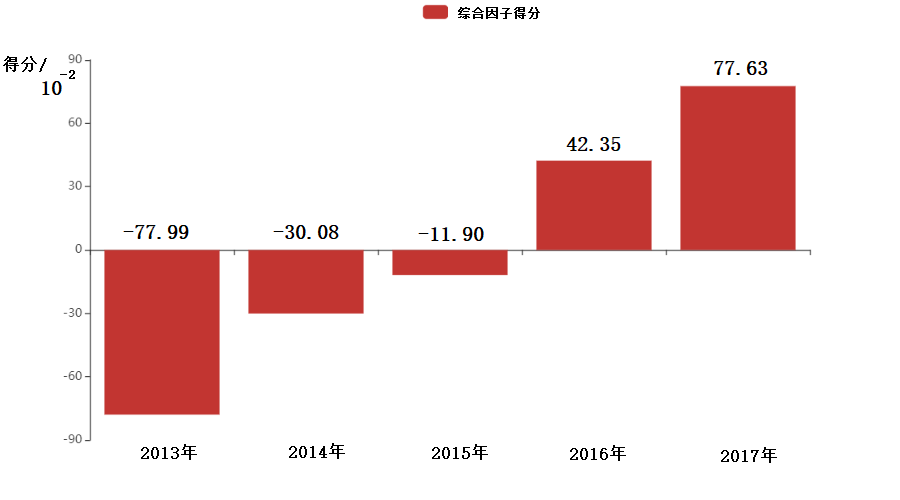
\includegraphics[width=\textwidth]{figures/wuhan.png}
		\caption{综合因子得分}
	\end{figure} 
	\subsection{结果分析}

	(1)人才吸引力的33个指标经因子分析和主成分分析后综合成的4个公因子,由回归法求得的图~\ref{defenyinzi}~、~\ref{fff}~所示,4个公因子的累计方差达到99.92\%,反应的信息量达到比较合适的比例。
	
	(2)根据武汉每年的因子得分表计算构建出的2013-2017年武汉综合因子得分表表明武汉市对于人才吸引力水平整体呈上升趋势,基本符合近几年武汉人才吸引力情况,说明武汉市对人才的吸引力随时间呈正向发展。
	
	(3)由表~\ref{cehngfenjuzheng}~至表~\ref{fff}~的分析数据显示,影响人才吸引力最主要因素是工业发展与薪酬因子,其次是医疗卫生环境因子,再者是经济贸易因子,最后是拥挤程度因子。从中可以看出,吸引人才的首先是一个地区发展前景和薪资水平的高低,,虽然地区交通拥挤程度也很重要,但对于个人而言,医疗卫生环境和经济贸易发展更为关键。
	
	(4)由表~\ref{xuanzhuanhuo}~可以看出,武汉市经济贸易因子和工业发展与薪酬因子逐年提高,这一方面与武汉市提出的《武汉市人力资源和社会保障事业发展"十三五"规划》有关,另一方面也与武汉市推进人才引进落户政策有关。近几年武汉市医疗卫生环境因子整体呈上升趋势,这归功于武汉市政府进一步加大对于专业技术人员的教育力度。
	

	
	
	\section{问题二模型的建立与求解}
	\subsection{问题的描述与分析}
	问题二要求针对具体人才类别,量化分析比较武汉市与其它同类城市的人才吸引力。本文在问题一模型的基础上改进,将人才分为三类\textbf{——}第一产业人才、第二产业人才和第三产业人才,并将问题一中的人才吸引力因素通过灰色相关度分成针对各类型人才的主要影响因素,再对分类后数据进行因子分析得到成都、天津、西安、南京和武汉2013—2017年分别对于三类人才吸引力的因子分析模型,并计算每个城市每年针对于三类人才的人才吸引力综合得分。 其分析流程图如图~\ref{2222}~所示:
	
	\begin{figure}[H]
	\centering
	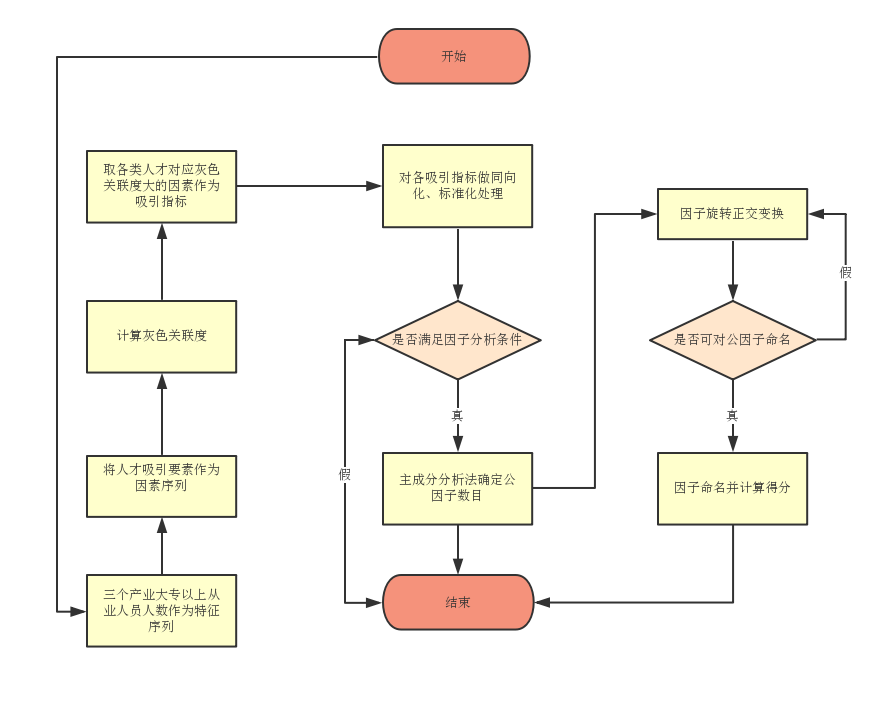
\includegraphics[width=\textwidth]{figures/2222.png}
	\caption{问题二分析流程图}\label{2222}
	\end{figure}



	\subsection{模型的建立与求解}

	\subsubsection{人才及其吸引力影响因素的分类}
	不同产业的人才会有不同的关注焦点,所以城市对不同产业类型的人才吸引力影响因素也存在差异。我们把人才分为三个类型\textbf{——}第一产业人才、第二产业人才和第三产业人才。通过查阅资料\cite{武汉统计局}收集了武汉2013—2017年第一、第二和第三产业大专以上从业人员人数,所收集数据得到表~\ref{hhh}~如下:
	\begin{table}[H]
		\centering
		\caption{各人才类别从业人数}\label{hhh}
		\begin{tabular}{cccc}
			\toprule[2pt]
			\multicolumn{1}{m{2cm}}{\centering 年份}&
			\multicolumn{1}{m{3cm}}{\centering 第一产业人才} & \multicolumn{1}{m{3cm}}{\centering 第二产业人才} & \multicolumn{1}{m{3cm}}{\centering 第三产业人才}\\
			\midrule[1pt]
			2013	 &  3800 & 1022800&958800\\ 
			2014 & 3571 & 1039720&980144\\ 
			2015	 &  3577&1046760&1022431\\ 
			2016  &  3466& 1053081&1076044\\ 
			2017  & 3229& 1037628&1158174\\
			\bottomrule[2pt]
		\end{tabular}
	\end{table}

	利用灰色关联度理论分别分析三类人才的$33$个影响因素,得到每个影响因子与用电量之间的关联度系数,具体步骤如下:
	确定因素序列和特征序列。本文分别以武汉2013—2017年第一、第二和第三产业大专以上从业人员人数作为特征序列,设为$x_{k}(p)$,采用$n(n=15)$个数据:$x_{k}(p)={x_{k}(1),x_{k}(2),···,x_{k}(5)}(k=1,2,3)$;将$33$个人才吸引要素作为因素序列,设为$x_{i}(t)$,其中有$m(m=33)$个子序列,每个子序列对应$5$个数据:$x_{i}(p)={x_{i}(1),x_{i}(2),···,x_{i}(5)}$。
	
	计算两极最小差 $k$和最大差$K$。计算出特征序列与因素序列的序列差为$\Delta _{i}(t)$,找到结果中的最小差和最大差。其中:
	\begin{gather}
	\begin{array} { l } { \Delta _ { 1 } ( t ) = \left| x _ { 0 } ( t ) - x _ { 1 } ( t ) \right| } \\ { k = \min \min \Delta _ { i } ( t ) } \\ { K = \max \max \Delta _ { i } ( t ) } \end{array}
	\end{gather}
	灰色关联系数和关联度。因素序列和特征序列在第$T$点的关联系数为:
	\begin{gather}
	\Phi _ { 0 , ( p ) } = \frac { k + \varepsilon K } { \Delta _ { 0 i } ( t ) + \varepsilon K }
	\end{gather}
	其中 $\varepsilon$为分辨系数,取$\varepsilon=0.5$。

	利用 MATLAB 软件分析计算后,取各类人才灰色关联度大小前十的影响因素作为其主要影响因素,如表~\ref{guan}~所示:
		\begin{table}[H]
		\centering
		\caption{各人才类别从业人数}\label{guan}
		\begin{tabular}{cccccc}
			\toprule[2pt]
			\multicolumn{1}{m{3cm}}{\centering 第一产业}&
			\multicolumn{1}{m{1.5cm}|}{\centering 关联度} & \multicolumn{1}{m{3cm}}{\centering 第二产业} & \multicolumn{1}{m{1.5cm}|}{\centering 关联度}&
			\multicolumn{1}{m{3cm}}{\centering 第三产业} & \multicolumn{1}{m{1.5cm}}{\centering 关联度}\\
			\midrule[1pt]
			经济增长率	 &  0.897 & 农业&0.862&第三产业占比&0.978\\ 
			旅游业 &  0.874&第二产业&0.807&邮政业&0.958\\ 
			第三产业占比	 &  0.840&客运量(万人)&0.787&旅游业&0.933\\ 
			固定资产总额&  0.827& 商品房销售价格&0.771&年末电话用户&0.925\\ 
			房地产和投资业  & 0.786& 工业和建筑业&0.756&剧场、影剧院&0.922\\
			职工平均工资  &0.728& 执业/助理医师&0.748&地区生产总值&0.921\\
			人均GDP(元/人)  & 0.719& 固定资产总额&0.742&年末邮政局数&0.915\\
			在岗职工平均工资  & 0.711& 年末邮政局数&0.737&固定资产总额&0.907\\
			地方财政内收入  & 0.643& 地方财政内支出&0.736&货运量(万吨)&0.902\\
			地方财政内支出&0.643& 邮政业&0.726&客运量(万人)&0.887\\
			地区生产总值&0.615&消费品零售总额&0.716&地方财政内收入&0.880\\
			\bottomrule[2pt]
		\end{tabular}
	\end{table}
	
	
	\subsubsection{分类型人才吸引力分析}
	将归类后所得的影响第一产业人才吸引力的$10$个影响因素在五个城市中2013—2017年的数据,使用SPSS进行因子分析,按照累积贡献率的原则提取公因子,以综合性指标来相对全面的反映出全体因子对第一产业人才吸引力的影响情况。按照主因子的提取原则,通过碎石图可看出可以用$3$个主因子来描述此$10$个因子的影响;再通过旋转后因子贡献率计算所得的城市各因子得分得到各城市每年的第一产业人才吸引力综合得分。其计算公式如下:
	\begin{gather}
	\mathrm { F } = \left( 48.328 \mathrm { F } _ { 1 } + 28.667 \mathrm { F } _ { 2 } + 12.283 \mathrm { F } _ { 3 } \right) / 89.277
	%(附结果计算公式)
	\end{gather}
	将得到的五个城市2013—2017年的综合得分绘制为折线图的到图~\ref{11}~如下所示:
	\begin{figure}[H]
		\centering
		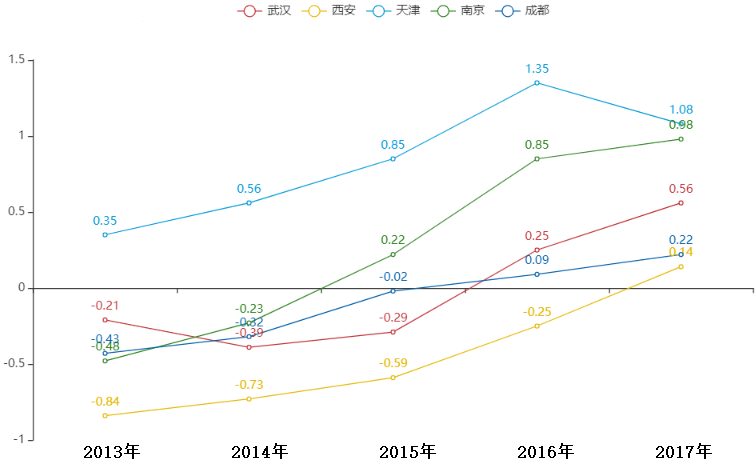
\includegraphics[width=.9\textwidth]{figures/11.png}
		\caption{第一产业人才吸引力综合得分折线图}\label{11}
	\end{figure} 
	同理将归类后所得的影响第二产业人才吸引力的$10$个影响因素使用SPSS进行因子分析,得到第二产业人才吸引力综合得分计算公式:
	\begin{gather}
	\mathrm { F } = \left( 27.594 \mathrm { F } _ { 1 } + 26.960 \mathrm { F } _ { 2 } + 16.609 \mathrm { F } _ { 3 } + 16.356 \mathrm { F } _ { 4 } \right) / 87.519
	%(附结果计算公式)
	\end{gather}
	第二产业人才吸引力综合得分折线图:
	\begin{figure}[H]
		\centering
		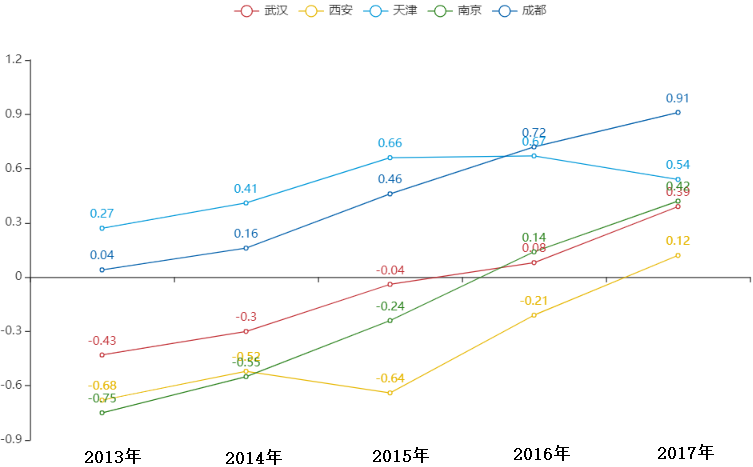
\includegraphics[width=.9\textwidth]{figures/22.png}
		\caption{第二产业人才吸引力综合得分折线图}\label{22}
	\end{figure}
	
	同理将归类后所得的影响第三产业人才吸引力的$10$个影响因素使用SPSS进行因子分析,得到第二产业人才吸引力综合得分计算公式:
	\begin{gather}
	\mathrm { F } = \left( 37.063 \mathrm { F } _ { 1 } + 25.130 \mathrm { F } _ { 2 } + 11.972 \mathrm { F } _ { 3 } + 10.477 \mathrm { F } _ { 4 } \right) / 84.642
	%(附结果计算公式)
	\end{gather}

	第三产业人才吸引力综合得分折线图:
		\begin{figure}[H]
		\centering
		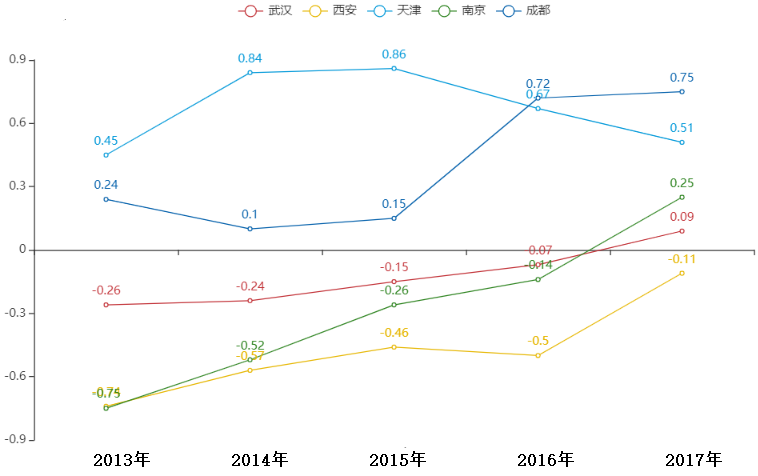
\includegraphics[width=\textwidth]{figures/33.png}
		\caption{第三产业人才吸引力综合得分折线图}\label{33}
	\end{figure}


	\subsection{结果分析}
	由图表可以看出,武汉市的人才吸引力水平近几年有较高的水平,尤其是对第二、三产业人才的吸引力表现出逐年增加趋势和较高水平,相对于西安和成都而言,武汉市具有较强的人才吸引力,十分符合地区的经
	济发展特点。而天津作为老牌北方直辖市,近年发展速度相比略显缓慢,导致其相应人才吸引力也有所下滑。
	
	但是,武汉在发展中也存在一些不足。特别是工业发展与薪酬因子处于人才吸引主导地位,而环境方面的因素尚未
	完全建立;优质教育与医疗资源分
	配不均、生活成本高、高校科研机构偏少等因素限制良好人才环境
	构建等。
	
	提高武汉市的人才吸引力水平,提出以下几点建议:
\begin{itemize}
	\item [(1)] 大力发展地方生产总值,为经济社会发展打下坚实的基础。
	\item [(2)]主要行业是加快人
	才发展的主导力量。建立较为高效的人才市场,通过各行业市场
	机制,人才较为充分地实现了自身价值,也为武汉的人才持续发展创
	造了良好条件。
	\item [(3)]注重整合空间结构全面发展,引导各大区块均衡协调稳步发展,
	建设全面型社会,注重生态建设,贯彻落实以人为本的科学发展理
	念。
	\item [(4)]加大营商环境改革力度,营
	造更加开放的贸易投资环境,营造综合成本适宜的产业发展环境,
	营造更加高效透明的政务环境。
	\item [(5)]政府不断完善就业服务政策,出台大量相关文件,高度重视高
	校毕业生的就业情况。
\end{itemize}

	\section{写给武汉市人力资源部门的建议报告}
	
	\section{模型的评价}
	\subsection{模型的优点}
	\begin{itemize}
		\item [(1)] 从国家统计数据库、武汉市统计年鉴和其他同类城市的统计年鉴中爬取大量数据,并挑选符合实际的33个指标与最近五年的数据进行评价。其吸引人才指标从多维度、全方面的考虑,具备科学性、客观性。
		\item [(2)]针对具体人才根据相应产业进行分类。相较于现有城市人才吸引力水平评价模型,我们采用了灰色关联分析法,对三种人才类别分析计算出与指标的相关系数,求出不同人才对33种影响因素的的偏好程度,选出前十个合适的指标进行综合打分。
	\end{itemize}

	
	\subsection{模型的缺点}
    未能具体地量化政府政策对人口吸引力的影响,只选取了地方财政收入、支出,固定资产投资总额三个影响因素作为政策影响的指标,与现实情况出现一定偏差,存在一定的局限性。

    
    
	\newpage	%换页符
	%%参考文献
	%\begin{thebibliography}{9}%宽度9
	% \setlength{\itemsep}{-2mm}
	\nocite{*}		%排版未引用的参考文献
\bibliography{wenxian.bib}
	%参考文献添加到wenxian.bib里,再引用
	
	\newpage
	%附录
	\appendix %%附录
\section{代码}
\subsection{数据预处理--python源代码}
\begin{lstlisting}[language=python]%这里修改语言
import pandas as pd
from sklearn.preprocessing import StandardScaler
from sklearn.decomposition import PCA
from factor_analyzer import FactorAnalyzer

#导入数据
df = pd.read_excel("wut.xls")
# print(df.head(5))

#转置
df = pd.DataFrame(df.values.T, index=df.columns, columns=df.index)
# print(df['商品房平均销售价格(元/平方米)'])

数据正向处理
df['商品房平均销售价格(元/平方米)'] = -(df['商品房平均销售价格(元/平方米)']-sum(df['商品房平均销售价格(元/平方米)'])/5)
df['工业废水排放量(万吨)'] = -(df['工业废水排放量(万吨)']-sum(df['工业废水排放量(万吨)'])/5)
df['工业二氧化硫排放量(吨)'] = -(df['工业二氧化硫排放量(吨)']-sum(df['工业二氧化硫排放量(吨)'])/5)
print(df['商品房平均销售价格(元/平方米)'])
print(df.head(5))
df.to_excel("武汉.xls")

#数据标准化
df = StandardScaler().fit_transform(df)
# print(df)
df=pd.DataFrame(df)
df.to_excel("武汉.xls")
#
#主成分分析
pca = PCA(n_components=4)
newX = pca.fit_transform(df)
print(newX)

#返回所保留的n个成分各自的方差百分比
print("它代表降维后的各主成分的方差值占总方差值的比例,这个比例越大,则越是重要的主成分")
print(pca.explained_variance_ratio_)
print("它代表降维后的各主成分的方差值,方差值越大,则说明越是重要的主成分")
print(pca.explained_variance_)

\end{lstlisting}


\end{document}